% Copyright (C) 2026 Vitor Mendes Camilo
% SPDX-License-Identifier: GPL-3.0-only
%
% This file is part of OpenJLS. Available under GPLv3 or a
% commercial license. See LICENSE and README for details.
%

% OpenJLS datasheet. Build: tectonic openjls_datasheet.tex
\documentclass[10pt,a4paper]{article}

\usepackage[margin=22mm]{geometry}
\usepackage{amsmath}
\usepackage{graphicx}
\usepackage{booktabs}
\usepackage{array}
\usepackage{tabularx}
\usepackage{xcolor}
\usepackage{enumitem}
\usepackage{ragged2e}
\usepackage{float}
\usepackage{caption}
\captionsetup{font=small,labelfont=bf,position=top,skip=6pt}
\usepackage{fancyhdr}
\usepackage{listings}
\usepackage{tikz}
\usepackage{tikz-timing}
\usepackage{hyperref}

\hypersetup{
    colorlinks=true,
    linkcolor=blue,
    filecolor=magenta,
    urlcolor=blue
  }


\graphicspath{{../Images/}}
\setlist{nosep,leftmargin=1.4em}
\newcolumntype{C}{>{\centering\arraybackslash}m{0.10\textwidth}}
\renewcommand{\arraystretch}{1.08}

\definecolor{ojblue}{RGB}{0,80,140}

\lstset{
  basicstyle=\ttfamily\scriptsize,
  keywordstyle=\color{ojblue}\bfseries,
  commentstyle=\color{gray},
  language=VHDL,
  showstringspaces=false,
  frame=single,
  columns=fullflexible,
}

\pagestyle{fancy}
\fancyhf{}
\lhead{\textbf{OpenJLS} — JPEG-LS Encoder IP}
\rhead{Datasheet}
\lfoot{\small v1.3}
\rfoot{\small \thepage}
\renewcommand{\headrulewidth}{0.4pt}

\setcounter{secnumdepth}{1}

\begin{document}

% wordmark PNGs carry ~9% transparent padding; the negative kern pulls the
% mark's ink flush with the right margin instead of the image box.
{\raggedleft\includegraphics[height=9mm]{isentropic-wordmark.png}\hspace*{-2.15mm}\par}

\vspace{3mm}

\begin{center}
  \includegraphics[height=20mm]{openjls-wordmark.png}\\[-2pt]
  {\large JPEG-LS Lossless Encoder IP Core --- Datasheet}
\end{center}

\vspace{4pt}

%======================================================================
\section{Overview}
OpenJLS is a JPEG-LS lossless encoder for FPGAs.
It encodes single-component (grayscale) images at one pixel per clock with no
external memory, streaming a standards-compliant JPEG-LS bitstream out over
a standard ready/valid streaming handshake. Source code, license and the full
verification suite are public at
\url{https://github.com/isentropic-fpga/OpenJLS}. There's also a companion public
repository with demo projects for OpenJLS at \url{https://github.com/isentropic-fpga/OpenJLS-Demos}.

\begin{table}[H]
  \centering
  \caption{Key specifications.}
  \label{tab:overview}
\begin{tabularx}{\textwidth}{@{}>{\bfseries}l X@{}}
  \toprule
  Standard      & JPEG-LS (ISO/IEC 14495-1, ITU-T T.87) \\
  Compression   & Lossless only \\
  Components    & Single (grayscale) \\
  Pixel depth   & 8--16 bits (\texttt{BITNESS}) \\
  Image size    & Up to $65535\times65535$ px\\
  Throughput    & 1 pixel / clock \\
  Latency       & 14 clock cycles \\
  $f_{max}$     & $\sim$280\,MHz (Xilinx \texttt{xczu7eg-1}) \\
  Interface     & Ready/valid streaming (AXI4-Stream / Avalon-ST compatible) \\
  Memory        & On-chip line buffer, one image row; no external RAM \\
  Resources     & $\sim$6.4k LUT, $\sim$2.0k FF + BRAM scaling with image width \\
  Portability   & Vendor-agnostic VHDL \\
  \bottomrule
\end{tabularx}
\end{table}

%======================================================================
\section{Revision and contact}
\begin{table}[H]
  \centering
  \caption{Revision history.}
  \label{tab:revision}
\begin{tabular}{@{}l l l@{}}
  \toprule
  \textbf{Version} & \textbf{Date} & \textbf{Notes} \\
  \midrule
  1.0 & 2026-06 & Initial release. \\
  1.1 & 2026-07 & Packaged IPs for Vivado. \\
  1.2 & 2026-07 & Isentropic branding; cores repackaged under the
  \texttt{isentropic} vendor. \\
  1.3 & 2026-09 & Byte-stuffer and prediction-error optimizations:
  frequency increased by $\sim$15\%, LUT reduction by $\sim$16\%,
  line-buffer BRAM up by $\sim$1 tile. \\
  \bottomrule
\end{tabular}
\end{table}

\noindent\textbf{License.} OpenJLS is dual-licensed: free under
\href{https://www.gnu.org/licenses/gpl-3.0.html}{GPL\,v3} for any GPL-compliant
use, or under a commercial license for proprietary products without GPL
obligations. Evaluation --- clone, simulate, synthesize, test --- is
unrestricted; a commercial license is required only to ship a product.

\noindent OpenJLS is developed and maintained by Isentropic. For commercial
licensing, technical questions, or collaboration inquiries, contact
\textbf{\href{mailto:contact@isentropic.com.br}{contact\allowbreak @\allowbreak isentropic.com.br}}.

%======================================================================
\section{Functional description}
The core is a fully pipelined encoder with a latency of 14 clock cycles: an
input register, six processing stages (gradient computation, context modeling,
MED prediction with bias correction, Golomb--Rice / run-length coding) and
three internally registered output stages (bit packer, byte stuffer, framer).

End-of-image is derived internally from the dimensions provided at the ports \texttt{iImageWidth} and \texttt{iImageHeight}.
The core never stalls --- neither at EOI (end of image) nor at EOL (end of line) --- which allows processing multiple images back-to-back.
The only exception is when the downstream stalls long enough for the byte-stuffer buffer to fill, which in turn stalls the upstream.

While the pipeline latency is 14 cycles, the core does not emit an output beat
every cycle: the output stages accumulate compressed bits and assert
\texttt{oValid} only once a full \texttt{OUT\_WIDTH} word is ready. As the
bitstream is compressed, these output beats are infrequent relative to the
one-pixel-per-clock input.

\begin{figure}[H]
  \centering
  \caption{Encoder pipeline architecture.}
  \label{fig:arch}
  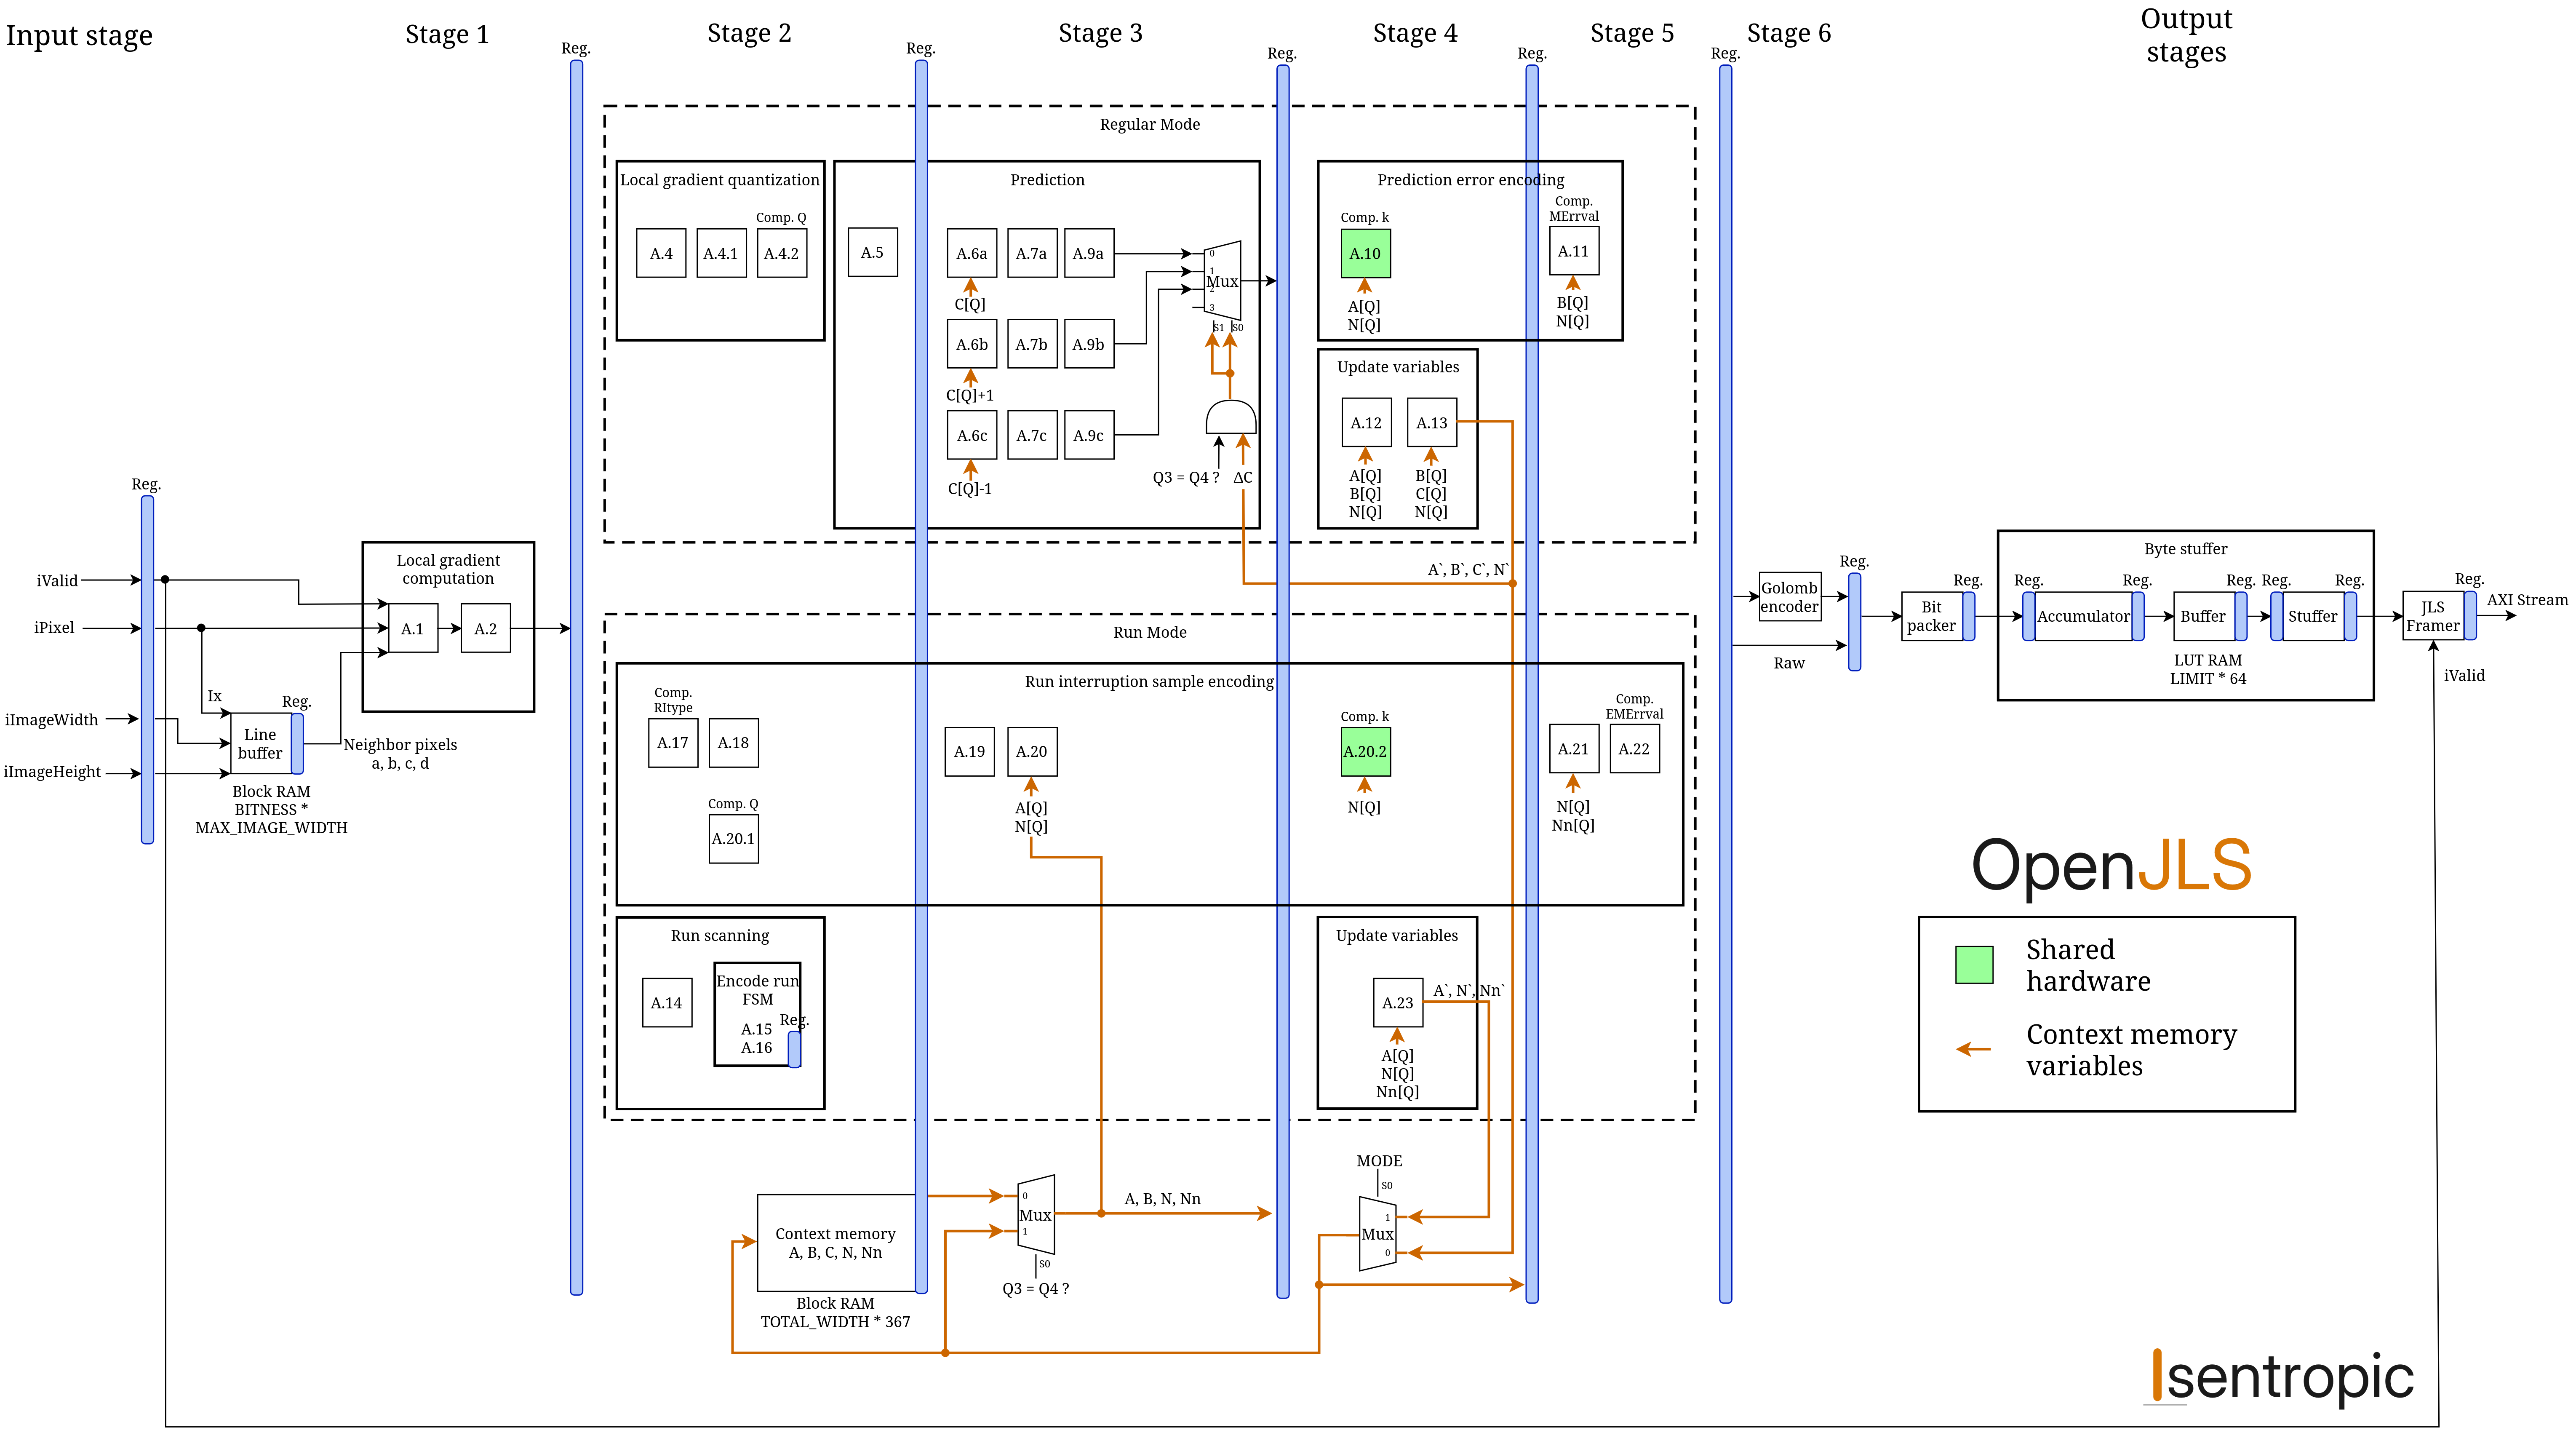
\includegraphics[width=\textwidth]{OpenJLS_arch.png}
\end{figure}

\noindent A \href{https://github.com/isentropic-fpga/OpenJLS/blob/main/Docs/Images/OpenJLS_arch.png}{full-resolution version} of this diagram is available in the
repository.

%======================================================================
\section{Generics}
The core is configured by the four generics in Table~\ref{tab:generics}.

\begin{table}[H]
  \centering
  \caption{Configuration generics.}
  \label{tab:generics}
\begin{tabularx}{\textwidth}{@{}l C X@{}}
  \toprule
  \textbf{Generic} & \textbf{Range} & \textbf{Description} \\
  \midrule
  \texttt{BITNESS}          & 8--16       & Pixel bit depth. \\
  \texttt{MAX\_IMAGE\_WIDTH}  & 4--65535    & Largest width supported; sets line-buffer depth. \\
  \texttt{MAX\_IMAGE\_HEIGHT} & 1--65535    & Largest height supported. \\
  \texttt{OUT\_WIDTH}        & 48--1024    & Output bus width in bits; multiple of 8. \\
  \bottomrule
\end{tabularx}
\end{table}

\noindent \texttt{MAX\_IMAGE\_WIDTH} and \texttt{MAX\_IMAGE\_HEIGHT} fix the
\emph{compile-time} maximum image size: they size the on-chip line buffer and the
dimension counters, so a larger maximum costs more BRAM. They do not select the
size of a given image --- the dimensions of each encoded image are chosen at
\emph{run time} through the \texttt{iImageWidth} and \texttt{iImageHeight} ports
(Table~\ref{tab:ports}), which accept any value from the minimum up to the
configured maximum.

%======================================================================
\section{Ports}
All ports are synchronous to the rising edge of \texttt{iClk} --- the core is a
single clock domain. The streaming
ports use a plain ready/valid handshake; in Table~\ref{tab:ports} the
\textbf{AXIS} column gives the one-to-one AXI4-Stream signal mapping for that
ecosystem (Avalon-ST maps the same way at \texttt{readyLatency}~=~0).

\begin{table}[H]
  \centering
  \caption{Port list and AXI4-Stream mapping.}
  \label{tab:ports}
\begin{tabularx}{\textwidth}{@{}l c l l X@{}}
  \toprule
  \textbf{Port} & \textbf{Dir} & \textbf{Width} & \textbf{AXIS} & \textbf{Role} \\
  \midrule
  \texttt{iClk}        & in  & 1                       & ---             & Clock. \\
  \texttt{iRst}        & in  & 1                       & ---             & Synchronous reset, active high; latches dimensions. \\
  \texttt{iImageWidth} & in  & 16                      & --- & Image width, pixels (configuration). \\
  \texttt{iImageHeight}& in  & 16                      & --- & Image height, pixels (configuration). \\
  \texttt{iValid}      & in  & 1                       & \texttt{TVALID} & Pixel valid. \\
  \texttt{iPixel}      & in  & \texttt{BITNESS}        & \texttt{TDATA}  & Pixel data. \\
  \texttt{oReady}      & out & 1                       & \texttt{TREADY} & Input ready. \\
  \texttt{oData}       & out & \texttt{OUT\_WIDTH}     & \texttt{TDATA}  & Bitstream beat. \\
  \texttt{oValid}      & out & 1                       & \texttt{TVALID} & Output valid. \\
  \texttt{oKeep}       & out & \texttt{OUT\_WIDTH/8}   & \texttt{TKEEP}  & Valid-byte mask on final beat. \\
  \texttt{oLast}       & out & 1                       & \texttt{TLAST}  & End of image. \\
  \texttt{iReady}      & in  & 1                       & \texttt{TREADY} & Downstream ready. \\
  \bottomrule
\end{tabularx}
\end{table}

\noindent \textit{IMPORTANT:}
\begin{itemize}
  \item \texttt{iImageWidth} and \texttt{iImageHeight} are only sampled while \texttt{iRst} is asserted (\texttt{'1'}).
  \item If an invalid value is provided to \texttt{iImageWidth}, that is \texttt{iImageWidth > MAX\_IMAGE\_WIDTH} or \texttt{iImageWidth < 4}, the encoder uses \texttt{MAX\_IMAGE\_WIDTH} as the image width.
  \item If an invalid value is provided to \texttt{iImageHeight}, that is \texttt{iImageHeight > MAX\_IMAGE\_HEIGHT} or \texttt{iImageHeight < 1}, the encoder uses \texttt{MAX\_IMAGE\_HEIGHT} as the image height.
  \item If you don't intend to change the image dimensions at run-time, wire both inputs to \texttt{0} so that the maximum values are used.
  \item Both ports are a fixed 16 bits regardless of the \texttt{MAX\_IMAGE\_*} generics --- every representable value is checked, so any out-of-range value is caught and replaced by the maximum.
\end{itemize}

%======================================================================
\section{Timing and protocol}

\textbf{Pixel input.} Pixels are streamed in scan order --- the first row left
to right, then the second row, and so on --- each an unsigned value on
\texttt{iPixel}. A pixel transfers on every cycle where
\texttt{iValid} and \texttt{oReady} are both high. The core asserts
\texttt{oReady} continuously and deasserts it only when the FIFO in byte stuffer fills
under downstream backpressure. Figure~\ref{fig:timing-input} shows a transfer
with a brief downstream stall.

\begin{figure}[H]
  \centering
  \caption{Pixel-input handshake.}
  \label{fig:timing-input}
\begin{tikztimingtable}[timing/slope=0.1,xscale=1.7]
  iClk    & 8{C}        \\
  iPixel  & D{P0} 4D{P1} 2D{P2} D{P3}\\
  iValid  & 8H          \\
  oReady  & HHLLHHHH     \\
\end{tikztimingtable}
\end{figure}
\noindent In Figure~\ref{fig:timing-input}, \texttt{P2} is held flat across the
stall and accepted when \texttt{oReady} returns high; no pixel is dropped while
\texttt{oReady} is low.

\textbf{Reset and configuration.} \texttt{iRst} is level-sensitive (hold it high
for at least one clock) and clears the pipeline. The image dimensions are
captured only while \texttt{iRst} is high: present \texttt{iImageWidth} and
\texttt{iImageHeight}, hold them stable across the reset pulse, and they latch on
the rising edge (Figure~\ref{fig:timing-reset}). A reset is therefore needed only
to capture the dimensions --- before the first image and whenever the image size
changes; with the size unchanged, images encode back-to-back.

\begin{figure}[H]
  \centering
  \caption{Reset and dimension capture.}
  \label{fig:timing-reset}
\begin{tikztimingtable}[timing/slope=0.1,xscale=1.45]
  iClk         & 7{C}          \\
  iImageWidth  & D{W0} 6D{W1}  \\
  iImageHeight & D{H0} 6D{H1}  \\
  iRst         & LLLHHLL        \\
  sImageWidth  & 5D{W0} 2D{W1} \\
  sImageHeight & 5D{H0} 2D{H1} \\
\end{tikztimingtable}
\end{figure}
\noindent In Figure~\ref{fig:timing-reset}, the new size (\texttt{W1}/\texttt{H1})
is driven for several cycles, then \texttt{iRst} pulses high; the dimensions
register on the rising edge while \texttt{iRst} is high.

\textbf{Output.} Beats appear on \texttt{oData}/\texttt{oValid} subject to
\texttt{iReady}; \texttt{oLast} marks the final beat (EOI) and \texttt{oKeep} flags
its valid bytes. The bitstream is byte-serial and MSB-first: the earliest byte
occupies the most-significant byte of \texttt{oData}. Pipeline latency is 14
clock cycles.

%======================================================================
\section{Resources and performance}
Characterized on Xilinx Zynq UltraScale+ \texttt{xczu7eg-fbvb900-1-e},
Vivado 2025.2, using the generics \texttt{BITNESS = 12} and \texttt{OUT\_WIDTH = 64}, RTL-only with no floorplanning.
$f_{max}$ is the true maximum, found by over-constraining the clock until timing fails.
At one pixel per clock, $\sim$280\,MHz is $\sim$280\,Mpixel/s.

\noindent Figure~\ref{fig:fmax} and Table~\ref{tab:fmax} report $f_{max}$ across
\texttt{MAX\_IMAGE\_WIDTH}; Figure~\ref{fig:util} and Table~\ref{tab:util} report
the resource usage.

\begin{figure}[H]
  \centering
  \caption{Maximum frequency vs maximum image width.}
  \label{fig:fmax}
  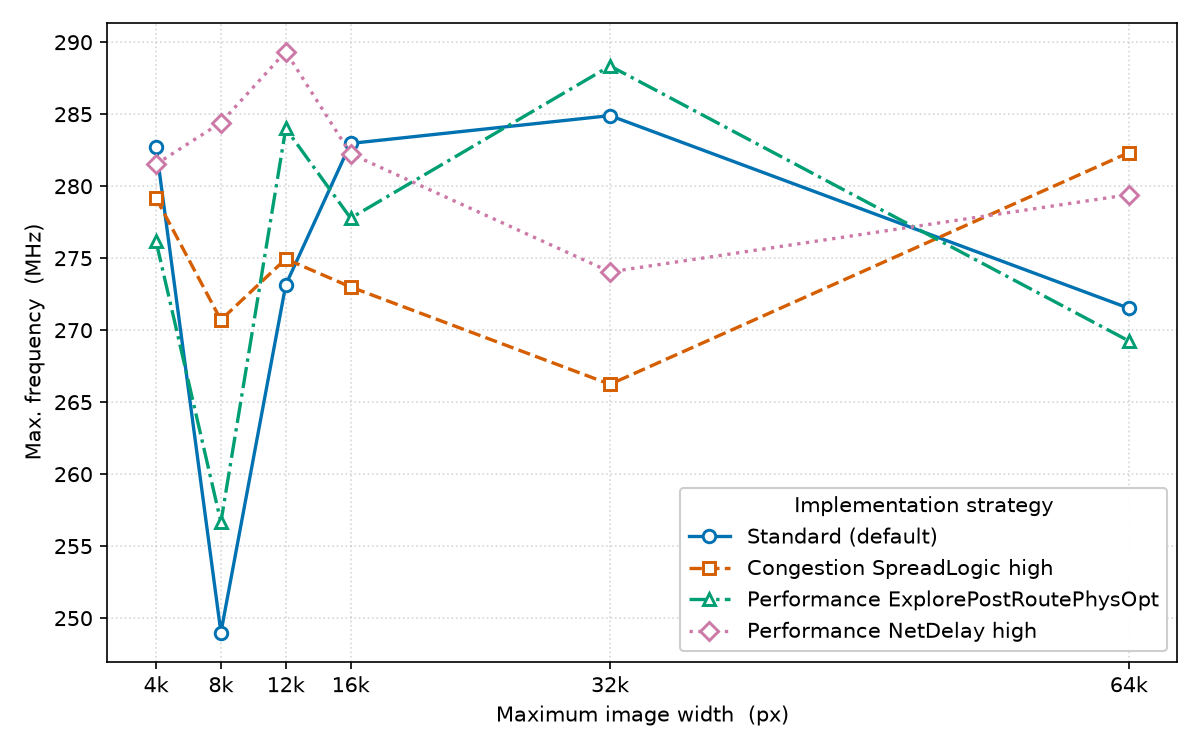
\includegraphics[width=0.70\linewidth]{fmax_vs_size.png}
\end{figure}

\begin{table}[H]
  \centering
  \caption{Maximum frequency by maximum image width and strategy.}
  \label{tab:fmax}
\begin{tabular}{@{}r @{\hspace{1.2em}}|@{\hspace{1.2em}} r r r r@{}}
  \toprule
  \texttt{MAX\_IMAGE\_WIDTH} & Default & EPRPO & NetDelay & Congestion \\
  \midrule
  4096  & \textbf{282.7} & 276.2          & 281.5          & 279.2          \\
  8192  & 249.0          & 256.7          & \textbf{284.4} & 270.7          \\
  12288 & 273.1          & 284.0          & \textbf{289.4} & 274.9          \\
  16384 & \textbf{283.0} & 277.8          & 282.2          & 273.0          \\
  32768 & 284.9          & \textbf{288.4} & 274.1          & 266.2          \\
  65535 & 271.5          & 269.2          & 279.4          & \textbf{282.3} \\
  \bottomrule
\end{tabular}
\end{table}

\begin{figure}[H]
  \centering
  \caption{Resource usage vs maximum image width.}
  \label{fig:util}
  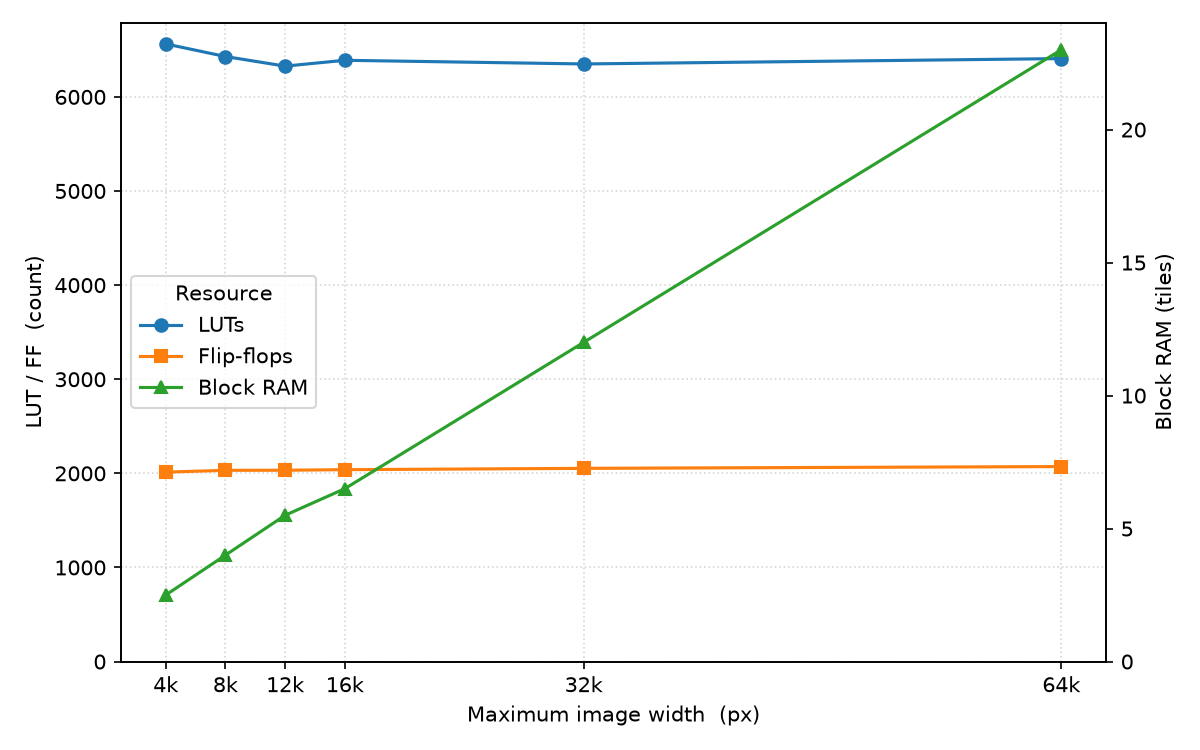
\includegraphics[width=0.70\linewidth]{util_vs_size.png}
\end{figure}

\begin{table}[H]
  \centering
  \caption{Resource usage by maximum image width.}
  \label{tab:util}
\begin{tabular}{@{}r @{\hspace{1.2em}}|@{\hspace{1.2em}} r r r@{}}
  \toprule
  \texttt{MAX\_IMAGE\_WIDTH} & LUT & FF & BRAM \\
  \midrule
  4096  & 6563 & 2013 & 2.5 \\
  8192  & 6429 & 2032 & 4.0 \\
  12288 & 6327 & 2033 & 5.5 \\
  16384 & 6389 & 2039 & 6.5 \\
  32768 & 6350 & 2053 & 12.0 \\
  65535 & 6407 & 2072 & 23.0 \\
  \bottomrule
\end{tabular}
\end{table}

\begin{sloppypar}
\noindent In Table~\ref{tab:fmax} frequencies are in MHz and the best strategy
per row is in bold; the strategies are \texttt{Performance\_\allowbreak Explore\allowbreak PostRoute\allowbreak PhysOpt}
(EPRPO), \texttt{Performance\_\allowbreak NetDelay\_\allowbreak high} (NetDelay) and
\texttt{Congestion\_\allowbreak SpreadLogic\_\allowbreak high} (Congestion). The design is congestion-bound,
so the winning strategy shifts with image size; a given netlist is deterministic,
but the per-size winner is placement-sensitive and can shift when the netlist
changes, so the best-of band ($\sim$282--289\,MHz) is the headline figure; the per-size spread across strategies is 7--22\,MHz, so a default run lands close to it at most sizes. Table~\ref{tab:util} is for the default
strategy; utilization is near-identical across strategies. Logic is essentially
constant with image size; only the line-buffer BRAM scales with width and pixel
depth.
\end{sloppypar}

%======================================================================
\section{Integration example}
\begin{lstlisting}
u_enc : entity work.openjls_top
  generic map (
    BITNESS          => 8,
    MAX_IMAGE_WIDTH  => 4096,
    MAX_IMAGE_HEIGHT => 4096,
    OUT_WIDTH        => 64 )
  port map (
    iClk         => clk,
    iRst         => rst,
    iImageWidth  => img_w,                -- latched on reset
    iImageHeight => img_h,                -- latched on reset
    iValid       => s_valid,              -- pixel stream (AXIS slave)
    iPixel       => s_data,
    oReady       => s_ready,
    oData        => m_tdata,              -- bitstream (AXIS master)
    oValid       => m_tvalid,
    oKeep        => m_tkeep,
    oLast        => m_tlast,
    iReady       => m_tready );
\end{lstlisting}

\noindent Being a single entity with standard ready/valid ports, \texttt{openjls\_top}
can equally be dropped onto a block diagram and wired there, instead of instantiating
it in HDL. The dimension ports are fixed at 16 bits (rather than sized from the
generics) because Vivado's block-design port-width evaluator only handles literal
arithmetic in port expressions.

\subsection{Xilinx IP cores}
For the Vivado flow the core ships the following pre-packaged IPs

\begin{table}[H]
  \centering
\begin{tabularx}{\textwidth}{@{}X X@{}}
  \toprule
  \textbf{IP Catalog name} & \textbf{Interfaces} \\
  \midrule
  OpenJLS Encoder (Native)                  & Plain Ready/Valid\\
  OpenJLS Encoder (AXI4-Stream)             & AXI-Stream for the data, native pins for control \\
  OpenJLS Encoder (AXI4-Stream + AXI4-Lite) & AXI-Stream for the data, AXI-Lite for control \\
  \bottomrule
\end{tabularx}
\end{table}

To use simply add \texttt{Sources/Xilinx/ip\_repo/} to the project's IP repositories
and the three cores appear in the
IP Catalog, ready to drop onto a block design.

\subsection{AXI4-Lite register map}
The AXI4-Lite variant replaces the native control pins with a register bank
(32-bit registers, word-aligned offsets):

\begin{table}[H]
  \centering
\begin{tabularx}{\textwidth}{@{}l l l X@{}}
  \toprule
  \textbf{Offset} & \textbf{Name} & \textbf{Access} & \textbf{Contents} \\
  \midrule
  \texttt{0x00} & ID      & RO & ASCII \texttt{"OJLS"} (\texttt{0x4F4A4C53}) \\
  \texttt{0x04} & VERSION & RO & \texttt{0x00MMmmpp} (major/minor/patch) \\
  \texttt{0x08} & CAPS    & RO & [7:0] \texttt{BITNESS}, [15:8] output bytes per beat (\texttt{OUT\_WIDTH}/8) \\
  \texttt{0x0C} & MAXDIM  & RO & [15:0] \texttt{MAX\_IMAGE\_WIDTH}, [31:16] \texttt{MAX\_IMAGE\_HEIGHT} \\
  \texttt{0x10} & WIDTH   & RW & [15:0] image width (clamped on write) \\
  \texttt{0x14} & HEIGHT  & RW & [15:0] image height (clamped on write) \\
  \texttt{0x18} & CTRL    & WO & [0] APPLY --- self-clearing, pulses the core reset \\
  \texttt{0x1C} & STATUS  & RO & [0] BUSY (reset pulse active), [1] pixel-stream TREADY mirror \\
  \bottomrule
\end{tabularx}
\end{table}

The core samples the dimensions only while its reset is high, so reconfiguration
is: write WIDTH/HEIGHT, set CTRL.APPLY. APPLY pulses the core reset for one clock
while the registers are held stable; the AXI-Lite endpoint itself stays on
\texttt{aresetn} only, so the bus never disappears mid-reconfigure. While the
pulse is active STATUS.BUSY reads 1 and the pixel stream's TREADY is held low, so
a stream started too early stalls instead of losing pixels --- WIDTH/HEIGHT/CTRL
writes while BUSY are dropped. Back-to-back images of unchanged dimensions need
no APPLY.

WIDTH/HEIGHT writes are merged per WSTRB and clamped to the core's rule
(out-of-range values become the MAX generic), so a readback always returns the
value the core will actually use. Writes to RO or unmapped offsets are
acknowledged (OKAY) and dropped; unmapped reads return zero.

\medskip
\noindent For driver code there is a C header in the repository,
\href{https://github.com/isentropic-fpga/OpenJLS/blob/main/Sources/Xilinx/ojls_regs.h}{ojls\_regs.h}.


%======================================================================
\section{Conformance and verification}
Verified by simulation with NVC using a layered, self-checking suite run at
both RTL and post-synthesis (gate-level) stages:
\begin{itemize}
  \item \textbf{OSVVM} --- Per-module tests against independent T.87-derived
        reference models, top-level control-plane stress (reset injection,
        backpressure, back-to-back images, dimension fallback), and AXI wrapper
        tests (byte-exact AXI4-Stream pass-through at 8- and 12-bit, AXI4-Lite
        register map, live reconfiguration, mid-image abort), all with
        requirements tracking.
  \item \textbf{Coverage} --- OSVVM functional coverage with NVC structural code coverage (99\%+ statements).
  \item \textbf{Golden model} --- Byte-exact vs the independent CharLS C++
        encoder over 287 real and synthetic images, plus ISO/IEC 14495-1 vectors.
  \item \textbf{Design contracts} --- Embedded PSL assertions (ready/valid handshake protocol, internal handshakes) on every run.
  \item \textbf{Post-synthesis} --- The stress test and a golden-model subset re-run on the synthesized netlist.
  \item \textbf{Hardware-in-the-loop} --- The full 287-image corpus encoded end-to-end on a PYNQ-Z2 FPGA and byte-compared against CharLS on real silicon. Produced in the demos repository \href{https://github.com/isentropic-fpga/OpenJLS-Demos}{OpenJLS-Demos} by the EncodeOverEthernet project.
\end{itemize}

\noindent Table~\ref{tab:regression} is the latest regression snapshot.

\begin{table}[H]
  \centering
  \caption{Latest regression snapshot.}
  \label{tab:regression}
\begin{tabularx}{\textwidth}{@{}l c c X@{}}
  \toprule
  \textbf{Suite} & \textbf{Status} & \textbf{Test/Cov} & \textbf{Summary} \\
  \midrule
  NVC code coverage       & info & 99.8\% & Per-DUT-file statement breakdown \\
  OSVVM suite             & PASS & 100\%  & 60 tests, 2\,877\,433 affirmations (module + top + AXI wrappers) \\
  Golden model            & PASS & 100\%  & 287/287 images byte-exact vs CharLS \\
  Post-synth OSVVM        & PASS & 100\%  & Control-plane stress on the gate-level netlist \\
  Post-synth golden model & PASS & 100\%  & 156/156 images byte-exact vs CharLS \\
  Hardware-in-the-loop    & PASS & 100\%  & 287/287 images byte-exact vs CharLS on PYNQ-Z2 silicon \\
  \bottomrule
\end{tabularx}
\end{table}



\vspace{10pt}
\noindent\textbf{References.}
ITU-T T.87 / ISO/IEC 14495-1;
Y.\,M.\,Mert, \emph{Key Architectural Optimizations for Hardware Efficient
JPEG-LS Encoder}, IEEE 2018;
\href{https://github.com/team-charls/charls}{CharLS};
\href{https://github.com/open-logic/open-logic}{open-logic}.

\end{document}
